\subsection{Richards Frequenztransformation}

Der  Frequenzbereich von konzentrierten LC-Filtern ist beschr\"ankt durch  die
Nichtidealit\"at der Komponenten.  W\"ahrend  die  Reaktanz und die G\"ute von
konzentrierten Induktivit\"aten und Kapazit\"aten  im  Bereich  \"uber  einige
\SI{100}{\mega\hertz} keinen hohen Filteranspr\"uchen mehr gen\"ugen k\"onnen,
w\"aren die entsprechenden Reaktanzen noch  sehr gut mit verteilten Elementen,
wie   leerlaufenden   und   kurzgeschlossenen  Leitungen  sowie  verschiedenen
gekoppelten   Leitungen  realisierbar.   Es   ist   beispielsweise   aus   der
Leitungstheorie  bekannt,  dass  leerlaufende  Leitungen   mit  einer  L\"ange
$l\le\frac{\lambda}{4}$   kapazitiv   und   kurzgeschlossene   Leitungen   mit
$l\le\frac{\lambda}{4}$  induktiv  sind.  Wir  k\"onnten damit die  induktiven
Reaktanzen und  die  kapazitiven  Suszeptanzen  mit  solchen Leitungselementen
ersetzen.

\begin{figure}
    \centering
    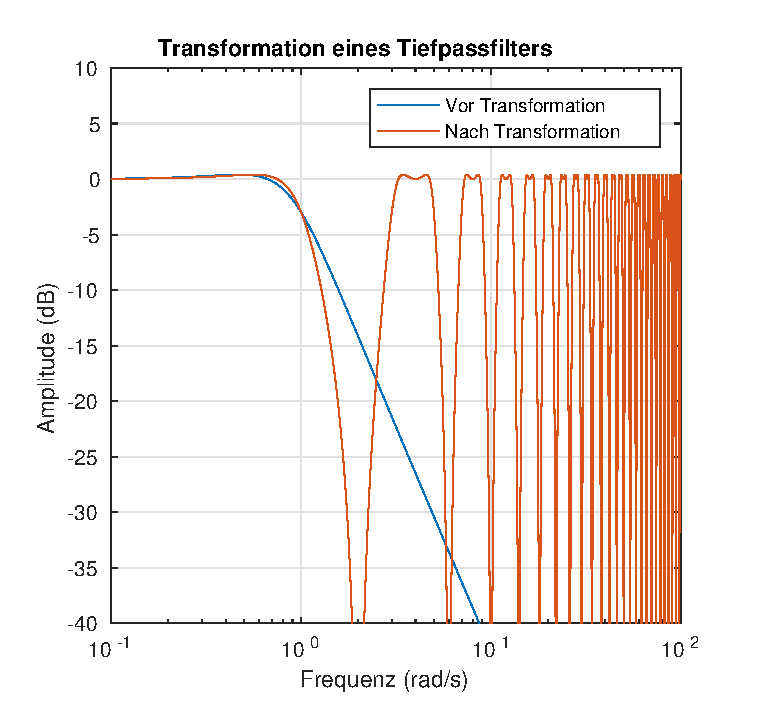
\includegraphics[width=\imagewidth]{images/richards-lowpass-example}
    \caption{Richards Frequenztransformation eines Chebychev-Tiefpassfilters (3. Ordnung)}
    \label{fig:richards-example}
\end{figure}

Dies wird mithilfe der sogenannten \textit{Richards Frequenztransformation} erreicht. 
